\chapter{Průzkum možných řešení}
Tato kapitola je zaměřena na hledání vhodného řešení zadaného problému. Vzhledem ke skutečnosti, že problém je dost specifický a nikdo jej ještě pomocí termokamery neřešil, jeho referenční řešení není známé. Jsou využity pouze znalosti získané při rešerši a je navrhnuto několik postupů, ze kterých bude vybrán ten nejvhodnější.

\section{Získávání dat z~kamery}
Před samotnou implementací algoritmů je nutné se zaměřit na získání dat. V~předchozí kapitole bylo popsáno, že se nejedná o~triviální úlohu a tak je potřeba vytvořit vlastní aplikaci pro nastavení a příjem dat z~kamery.

	\subsection{Aplikace pro přenos dat a komunikaci s~kamerou}
    V~rámci tvorby aplikace pro komunikaci s~kamerou, bylo nutné se seznámit s~poskytovaným rozhraním vybraného eBUS SDK. Dokumentace k~tomuto SDK je velmi detailní a tato část probíhala bez větších potíží. Bylo velmi snadné vytvoření jednoduché aplikace v~jazyce C++ pro připojení kamery, jejího nastavení a získání jednotlivých snímků. Problém nastal až při implementaci kontinuálního ukládání dat, kdy přes veškerou snahu se nedařilo tuto funkčnost zprovoznit. Aplikace se zasekávala, vracela chybová data a ukládání fungovalo nespolehlivě.
    
    Pro vypořádání se s~tímto problémem byla zvolena alternativa, a to využití aplikace eBUS Player z~ukázkových C++ kódů. Tato aplikace již obsahuje všechny nutné funkcionality pro správu připojení, nastavení a ukládání dat kamery. Bylo by možné pomocí této aplikace pouze data přenášet z~kamery, ukládat na disk a další práci nad daty provádět formou záznamu. Jako elegantnější řešení bylo rozšíření eBUS Playeru pro přenos dat do libovolného programovacího jazyka pomocí síťových soketů. Následné zpracování a třídění přenesených dat pak může probíhat pohodlněji ve vyšším programovacím jazyce. 
    
    V~této rozšířené aplikaci je možné nastavit všechna potřebná nastavení kamery pomocí uživatelského rozhraní a navázat komunikaci s~klientem. V~případě, že je komunikace navázána úspěšně, začnou se přijímaná data z~termokamery přenášet skrz soket. Při přenosu se nevyužije naplno propustnost síťového rozhraní, takže přenos není zahlcen a data klientem mohou být přijímány prakticky ihned. Obraz je tímto způsobem možné přenášet téměř v~reálném čase.
    
    Nutno podotknout, že součástí odesílaných souborů nejsou žádná metadata ani jiné hlavičky, které by popisovaly příchozí soubory. V~rámci práce to nebylo nutné, protože klientská aplikace vždy ví, jaká data má očekávat. 

	\subsection{Formát přenášených dat} \label{transmitted_data_format}    
    Aplikace pro příjímání dat z~kamery umožňuje ukládat data buď v~komprimovaných formátech jako je JPG a BMP, nebo v~nekomprimovaných jako je TIFF a nebo v~surovém formátu, kde jsou obsahem jednotlivé hodnoty z~detektoru. Vzhledem k~tomu, že je vždy lepší pracovat s~co nejméně komprimovanými daty, je rozhodnuto pro přenos surových dat. Tato nezpracovaná data je z~termokamery možné přijímat ve dvou různých formátech. To se řídí dle nastaveného režimu v~protokolu GenICam.
       
    \begin{description}[align=left]\label{description:transfer_data_modes}
      \item [Signal linear mode] V~tomto režimu odpovídají jednotlivé pixely obrazu hodnotám signálu z~maticového detektoru. Tento signál toho sám o~sobě nic moc neříká, může být pouze převeden na teplotu. Pro převod signálu S~na teplotu T v~kelvinech slouží vzorec:

      \begin{equation}
      	T_{[K]}=\frac{B}{\ln{\left(\frac{R}{S - O} + F\right)}},
      \end{equation}

      kde hodnoty R, B, F, O~jsou uloženy v~registrech kamery a lze je zjistit v~uživatelském rozhraní přehrávače eBUS a nebo dotazem do GenICam protokolu.

      \item [Temperature linear mode]\label{item:temperature_linear} Data získaná v~tomto režimu při vynásobení konstantou $K$ přímo odpovídají teplotám. Hodnota konstanty $K$ se liší dle typu kamery a také dle rozlišení signálu nastaveného v~protokolu GenICam. Pro kameru A65 teplotu $T$ v~kelvinech lze ze signálu $S$ získat jako:
      \begin{equation}
		T_{[K]}=0.04 \times
S~\end{equation} 
      
      pro vysoké rozlišení signálu a 
      
      \begin{equation}
		T_{[K]}=0.4 \times
S~\end{equation}
       
       pro nízké rozlišení signálu.
    \end{description}
    
    Z~výše uvedených způsobů získání teplot ze surových dat je zřejmé, že využití režimu Temperature linear je výpočetně jednodušší a pohodlnější, protože není potřeba dotazovat protokol a používat výpočetně náročný vzorec s~dělením a logaritmem pro každý pixel obrazu.   
    Přenášená data jsou tedy vždy odesílána neupravena, v~14-bitové kvalitě a ve formátu Temperature linear s~vysokým rozlišením.
    
	\subsection{Oblast snímání}
  	Nemělo by smysl snímat celé obrazové pole, protože se v~něm vyskytuje regál i osoba. V~tomto případě je zajímavé se zaměřit pouze na oblast, kde se může vyskytovat ruka. To znamená, snímat pouze bezprostřední oblast před regálem.

      Velikost této oblasti byla experimentálními způsoby stanovena pro obě kamery na hodnotu 640 $\times$ 150 pixelů. Oblast je záměrně o~něco širší než by bylo potřeba. Je to z~toho důvodu, že během snímání může kdykoliv nastat kalibrace NUC a přerušit tím snímání. Tím, že bude oblast o~něco větší, bude získáváno více snímků ruky a tím snížena pravděpodobnost, že NUC překazí snímání v~důležitý moment. 
      
      V~případě, že by kamera (13 mm) měla rychlejší snímkovací frekvenci, byla by pro ni oblast s~výškou 70 pixelů dostačující. Příklad výřezu oblasti a jeho neupraveného zdroje je zobrazen na obrázku \ref{fig:camera_2_sample_image_small} a \ref{fig:camera_2_sample_image_full}.
    
    \begin{figure}[h]
      \centering
      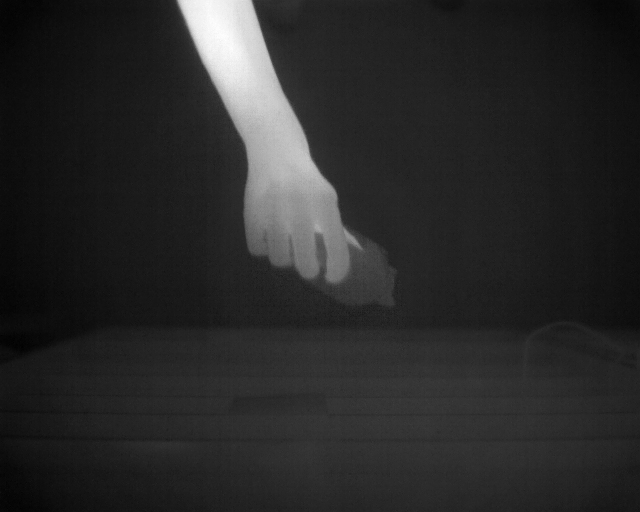
\includegraphics[width=0.8\textwidth]{images/camera_2_sample_image_full.jpg}
      \caption{Neupravený snímek v~plné velikost}
      \label{fig:camera_2_sample_image_full}
    \end{figure}  

    \begin{figure}[h]
      \centering
      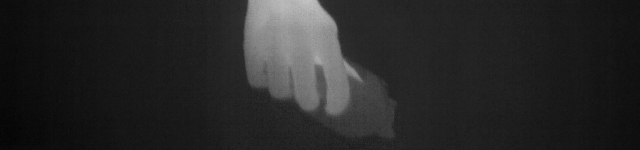
\includegraphics[width=0.8\textwidth]{images/camera_2_sample_image_small.jpg}
      \caption{Výřez oblasti zájmu neupraveného snímku}
      \label{fig:camera_2_sample_image_small}
    \end{figure}  

	\subsection{Redukce oblasti}\label{section:area_reduction}
    Kamera A65 v~sobě mimo jiné nese registry pro možnost snímání pouze výřezu obrazového pole. Díky tomu je možné z~kamery rovnou přijímat redukovanou oblast. Tyto registry se nastavují v~protokolu GenICam a je možné je změnit v~uživatelském rozhraní upraveného eBUS Playeru. Registry pro výběr oblasti jsou označeny jako: Width, Height, OffsetX, OffsetY. Jejich hodnoty pro jednotlivé kamery použité v~práci jsou uvedeny v~tabulce \ref{table:region_of_interest_settings}. Posun v~ose Y je nastaven tak, aby se zaznamenávaná ruka na snímku vyskytovala přibližně uprostřed.

    \begin{table}[h]
      \centering
      \begin{tabular}{|c|c|c|}
        \hline
        \rowcolor{Blue}
        \color{White}\textbf{Parametr} & \color{White}\textbf{Kamera 1 (13 mm)} & \color{White}\textbf{Kamera 2 (25 mm)}\\ \hline
        šířka & \multicolumn{2}{|c|}{640 pixelů}   \\ \hline
        výška & \multicolumn{2}{|c|}{150 pixelů}   \\ \hline
        posun v~ose X & \multicolumn{2}{|c|}{ 0 pixelů} \\ \hline
        posun v~ose Y & 190 pixelů & 170 pixelů \\ \hline
      \end{tabular}
      \caption{Hodnoty registrů pro výběr oblasti zájmu}
      \label{table:region_of_interest_settings}
    \end{table}
    
    Vyhotovení výřezu obrazového pole rovnou na straně termokamery je výhodné v~tom, že je přenos oproštěn od nezajímavých dat a není zbytečně zatěžováno síťové rozhraní. Pokud by se přeci jen přenášel celý snímek, musela by určitá redukce obrazového pole stejně proběhnout na straně klientské aplikace, protože většina algoritmů má velkou výpočetní náročnost a není nutné je provádět nad obrazem v~plném rozlišení.

  	\subsection{Proces snímání}
 	Snímání probíhalo v~Laboratoři zpracování obrazu na FIT ČVUT v~Praze. Teplota se v~této místnosti pohybovala v~rozmezí běžné pokojové teploty a to mezi 19 - 24 \textdegree{}C. Teplota zboží v~regále a podlahy v~podobných relacích. 
 
	Regál je vysoký 200 cm a široký 80 cm. Vzdálenost umístění kamer od země je uvedena na obrázku \ref{fig:shelf_scheme}. Reálné umístění kamery a podoba regálu je vidět na fotografii \ref{fig:shelf_setup}. Kamera je umístěna v~souladu s~posunem uvedeným v~\ref{section:area_reduction}, aby se ruka sahající do regálu vyskytovala přibližně uprostřed, kde obraz dosahuje nejvyšší kvality. Optika kamery je manuálně zaostřena přibližně do 3/4 regálu vzdálenosti od podlahy. 

  \begin{figure}[h]
    \centering
    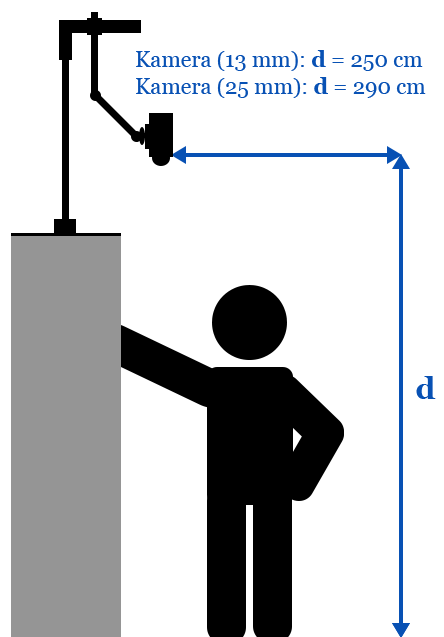
\includegraphics[width=0.5\textwidth]{images/camera_setup_scheme.png}
    \caption{Schéma umístění kamery}
    \label{fig:shelf_scheme}
  \end{figure}  

  \begin{figure}[h]
    \centering
    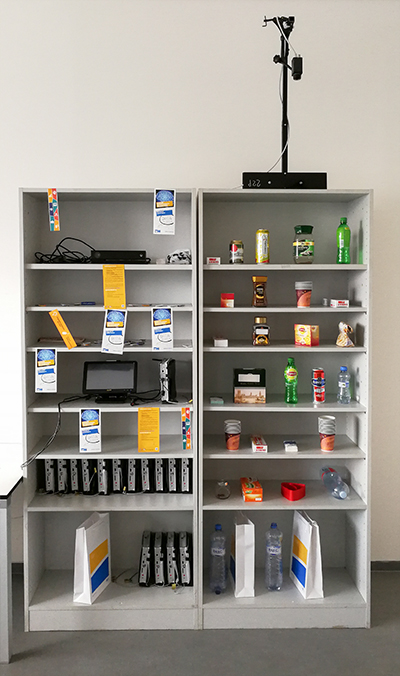
\includegraphics[width=0.6\textwidth]{images/shelf_setup.jpg}
    \caption{Fotografie umístění kamery}
    \label{fig:shelf_setup}
  \end{figure}    

\section{Předzpracování dat}
Ještě před začátkem aplikace algoritmů je data nutné převést z~binární podoby na teploty. Tyto teploty normalizovat do nového rozsahu, aby je bylo možné zobrazit. Poté už je možné pracovat se snímkem, který je nutno obrazově předzpracovat. 

Zpracování snímku probíhá v~následujícím pořadí: převod binárních dat, normalizace teplot, expoziční úpravy, odstranění šumu. Efekt těchto kroků je zobrazen na obrázku \ref{fig:camera_2_image_preprocessing}. 

\begin{figure}[h]
  \centering
  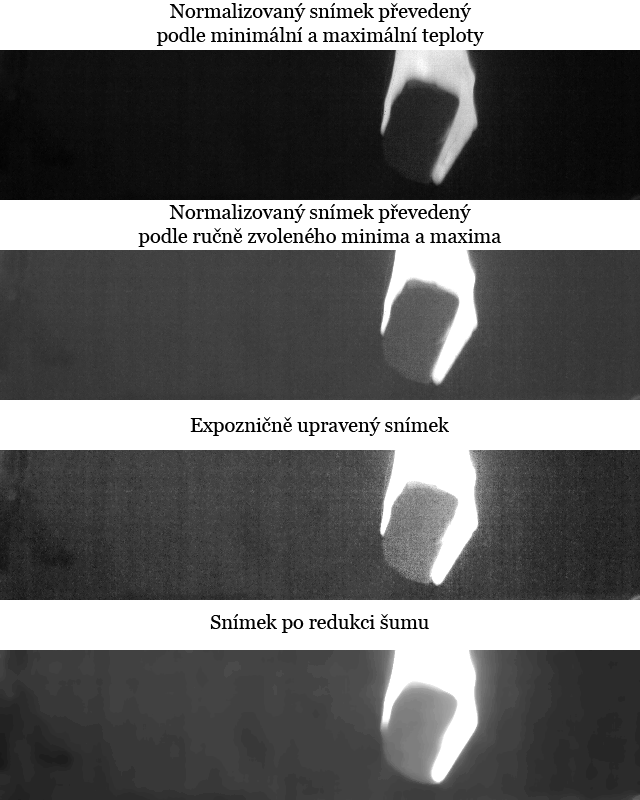
\includegraphics[width=0.8\textwidth]{images/camera_2_image_preprocessing.png}
  \caption{Jednotlivé kroky předzpracování snímku}
  \label{fig:camera_2_image_preprocessing}
\end{figure} 

	\subsection{Převod binárních dat a normalizace teplot}
    Binární data z~kamery jsou snímána v~Temperature linear režimu, takže je možné je snadno převést podle \ref{item:temperature_linear} na teplotu v~kelvinech. Teplotu v~kelvinech je ještě vhodné převést na běžnější teplotu v~\textdegree{}C a to pomocí jednoduchého vzorce:
    
    \begin{equation}
 	   T_{[C]}= T_{[K]} - 273.15,  
    \end{equation}
    
	kde $T_{[C]}$ je nová teplota v~\textdegree{}C a $T_{[K]}$ teplota v~K.
    
    Tyto teplotní data je nutné normalizovat do nového rozsahu, aby bylo možné je rozumně zobrazit. Nejjednodušším způsobem je ve snímku vyhledat minimální a maximální teplotu a všechny teploty normalizovat pomocí vzorce:
    
    \begin{equation}
  	  x_{norm} = \frac{(newMax - newMin) }{ (oldMax - oldMin)}* (x - oldMax) +newMax,
    \end{equation}
    
    kde $x$ je hodnota před normalizací, $x_{norm}$ je nová hodnota, $oldMax$ a $oldMin$ jsou nalezené minimální a maximální teploty v~snímku a $newMax$ a $newMin$ je nový rozsah hodnot. Většina algoritmů z~knihovny OpenCV pracuje pouze s~8-bitovými maticemi, takže je vhodné data převádět rovnou do 8-bitové podoby. Z~toho plyne, že hodnota $newMax$ je vždy 255 a $newMin$ vždy 0.
    
    Způsob normalizace snímku pomocí nalezené minimální a maximální teploty se ukázal jako nevhodný, protože zboží bylo stěží rozeznatelné i pro člověka. Hledání hodnot $oldMax$ a $oldMin$ tedy není automatizováno a jejich volba probíhá ručně.
   	
    \subsection{Úprava expozice a odstranění šumu}
    Normalizovaný snímek je pro zvýraznění teplotních rozdílů expozičně upraven. Proběhne zvýšení kontrastu a následné snížení jasu. Tímto procesem se na snímku vygeneruje velké množství šumu, které je potřeba zredukovat.
    
    Šum je odstraněn nejprve pomocí mediánového filtru \cite{huang1979fast} a následně ještě pomocí bilaterálního filtru \cite{tomasi1998bilateral}, který zachovává hrany.
    
\section{Řešení segmentací na základě teplot objektů} 
Prvním navrženým řešením je segmentace obrazu pouze na základě teplot. Toto řešení se dá považovat za velmi naivní, ale nemusí být hned jasné, v~čem spočívá problém.

Ještě před zpracováním snímku je možné z~jednotlivých pixelů získat konkrétní teploty. V~oblasti zájmu se může objevit pouze ruka, zboží a podlaha. Pro zamýšlení se nad dalším postupem je nutné zjistit rozmezí teplot těchto tří objektů.

Teplotně se ruka pohybuje přibližně od 26 \textdegree{}C a není zde moc co vymýšlet. Problém nastává s~určením rozsahu teploty zboží. Zboží se totiž v~průběhu manipulace zahřívá od ruky a nebo naopak ochlazuje okolním vzduchem. Pokud se teplota v~místnosti změní, některé zboží na tuto změnu reaguje rychleji a některé pomaleji v~závislosti na tepelné vodivosti. Zboží má oproti podlaze teplotu průměrně o~0.2 - 0.5 \textdegree{}C vyšší, ale může se stát, že některé zboží bude mít v~některých chvílích i nižší teplotu než má podlaha (díky tepelné vodivosti a změně teploty vzduchu). 

Dalším faktorem je nestabilita výstupu z~termokamery. Mezi jednotlivými korekcemi NUC (\ref{section:nuc}) se teplota s~postupem času nelineárně mění. Tento posun může být v~některých situacích až 1 \textdegree{}C za minutu. 

Najít přesný teplotní rozsah pro zboží není možné a tato úloha se tímto způsobem řešit nedá.

\clearpage

\section{Řešení s~využitím hranové detekce}\label{section:edge_detection_solution}
Druhým navrženým řešením je využít hranovou detekci pro získání hran objektu a prahování pro získání ruky. Prvním krokem je získání masky ruky z~předzpracovaného snímku. Masku je možné získat více způsoby. Byly experimentálně vyzkoušeny tyto postupy: binární prahování, Otsu prahování, adaptivní prahování, segmentace pomocí hranové detekce. Ukázalo se, že čím složitější metoda byla využita, tím byly výsledky horší, protože tyto adaptivní algoritmy se pro povahu úlohy nehodí. 

Pokud předzpracovaný snímek obsahuje ruku, tak si lze na obrázku \ref{fig:camera_2_image_preprocessing} všimnout, že pixely ruky jsou velmi jasné. Začínají průměrně od hodnoty 180 (v~rozmezí 0 černá a 255 bílá) a je snadné je rozlišit od tmavého pozadí. Pro získání masky ruky je  využito jednoduché, ale velmi rychlé, binární prahování s~hodnotou prahu 180.

Na snímku je dále patrné, že kolem ruky vzniká záře, která nenese žádnou informaci a lze ji považovat za šum. Tento šum se dá velmi obtížně redukovat, protože vzniká kolem celé oblasti ruky a ovlivňuje i zboží. Alespoň pro částečné odstranění této záře je využito morfologické operace dilatace \cite{serra1982image} s~obdélníkovým jádrem. Je však nutné počítat s~tím, že dilatace zmenšuje oblast pro zboží.

Aby byly hledány pouze relevantní hrany, je na snímku vyhledána oblast zájmu a ohraničena pomocí ohraničujícího obdélníku (bounding boxu). Oblast zájmu je nalezena pomocí vyhledání největší kontury. Pomocí největší kontury se pak řídí šířka oblasti, která je ještě vhodně zvětšena. Výška oblasti je vždy celá velikost snímku, protože zboží dost často přesahuje právě před rukou. Pokud není tato oblast nalezena, ruka se na snímku nevyskytuje a nemá smysl dále vyhodnocovat.

V~případě, že je nalezena oblast zájmu, je dalším krokem vyhledání hran. Stejně jako u~způsobu segmentace ruky bylo pro detekci hran experimentálně vyzkoušeno několik detektorů (Prewittův, Sobelův, Sacharrův, Laplaceův, Cannyho) s~různými způsoby nastavení a předzpracování obrazu. Ve všech případech poskytoval Cannyho hranový detektor \cite{canny1986computational} nejpřesnější výsledky. V~případech velmi malé jasové změny (teplota zboží blízko teplotě podlahy), nacházel též Cannyho detektor nejrelevantnější hrany.

Na nalezené hrany je dále v~několika iteracích aplikována dilatace a eroze pro spojení blízkých hran a odstranění hran malých, které jsou pravděpodobně šum. 

Výsledný snímek hran zboží vznikne jako binární součet snímku hran a~inverze binární masky ruky. Na tomto snímku se pak vypočtou předem dané atributy kontur (uvedeny v~následující kapitole \ref{section:attributes}), podle kterých je možné ho klasifikovat. Algoritmus je též graficky znázorněn ve vývojovém diagramu \ref{fig:edge_detection_diagram}.

\begin{figure}[h]
  \centering
  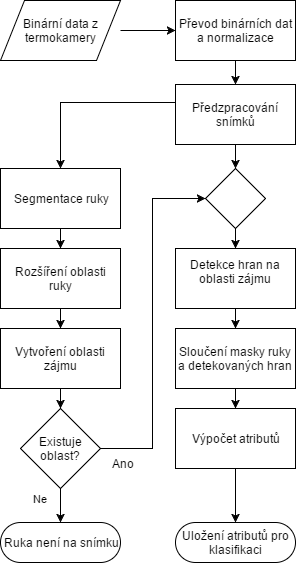
\includegraphics[width=0.6\textwidth]{images/edge_detection_diagram.png}
  \caption{Vývojový diagram algoritmu s~využitím hranové detekce}
  \label{fig:edge_detection_diagram}
\end{figure} 

    \subsection{Problémy}
    Toto řešení se mimo jiné ukázalo jako velmi citlivé na pohyb ruky. V~případě, že se ruka pohybuje rychle, na snímku se projeví pohybová neostrost, která díky nižší jasové hodnotě než má ruka, není segmentována. Následně se po aplikaci Cannyho detektoru jeví artefakty pohybové neostrosti ruky jako hrany zboží a tyto snímky jsou chybně klasifikovány. Problém s~nadbytečnými hranami způsobuje i záře, která se vyskytuje kolem ruky.

	\subsection{Vyhodnocení}
    Výsledky tohoto řešení se pohybovali v~rozmezí 65 - 75 \% celkové přesnosti klasifikace v~závislosti na použitém klasifikátoru. Detailnější informace nejsou dále diskutovány, protože toto řešení nebylo shledáno jako konečné a bylo navrženo lepší, které je následně detailněji vyhodnoceno.
         
\clearpage

\section{Řešení pomocí dynamického odčítání pozadí} \label{section:background_substract_solution}
Toto řešení bylo s~využitím nových znalostí a postřehů navrženo pro zlepšení předchozích výsledků. %Obsahuje více kroků, než předchozí řešení a jednotlivým metodám jsou parametry nastaveny experimentálně %Řešení využívá více různých po sobě jdoucích operací, které byly experimentálně nastaveny parametry, které byly nalezeny a shledány jako nejlepší kombinací.

V~paměti je uchováváno průběžně aktualizující se pozadí. Je to z~důvodu, že obraz z~termokamery není plně stabilní a mezi jednotlivými snímky se v~čase mění. Největší změna v~obraze se vždy projeví po  kalibraci NUC a je na ni nutné co nejrychleji reagovat. Z~toho důvodu nebylo použité pouze průměrování pozadí, ale je využito akumulovaní pozadí s~předem danou váhou. Při akumulovaní pozadí jsou jednotlivé pixely nového pozadí vypočteny jako:

\begin{equation}
	acc(x, y) = (1 - \alpha) \times acc(x, y) + a \times src(x,y),
\end{equation}

kde src(x, y) je hodnota vstupního pixelu na souřadnicích (x, y), acc(x, y) je hodnota pixelu akumulovaného pozadí v~paměti a $\alpha$ je váha nového pixelu. Čím větší je $\alpha$, tím je schopné se pozadí rychleji adaptovat na změnu prostředí. Pro $\alpha$ byly testovány hodnoty od 0,1 až do 0,5 a nakonec se pro tento typ úlohy ukázala jako nejlepší hodnota 0,3.

Od aktuálního snímku je odečteno pomocí \cite{opencvMOG} průběžně aktualizující se pozadí a z~této operace vznikne maska popředí. Tato maska je použita k~získání reálného popředí. Na získané popředí je stejně jako v~řešení \ref{section:edge_detection_solution} aplikováno binární prahování pro zisk masky ruky a tato maska je dilatací rozšířena. V~případě, že žádná maska ruky neexistuje, je snímek použit pro výpočet nového pozadí. Efekty těchto kroků je možné vidět na obrázku \ref{fig:camera_2_mog_preprocessed_substracted_hand}.

\begin{figure}[h]
  \centering
  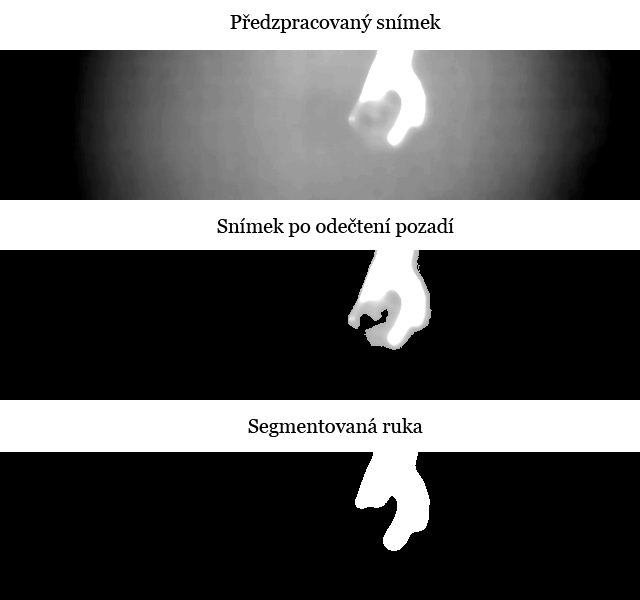
\includegraphics[width=0.8\textwidth]{images/camera_2_mog_preprocessed_substracted_hand.png}
  \caption{Ilustrace operací získání popředí snímků a segmentace ruky}
  \label{fig:camera_2_mog_preprocessed_substracted_hand}
\end{figure} 

Maska ruky je invertována a použita pro maskování popředí. Tímto způsobem na snímku zůstane šum a možné zboží, které je nutné nějakým způsobem zpracovat. Prvním aplikovaným způsobem je odstranění možného zboží od šumu ve formě záře kolem ruky. Tento postup spočívá v~nalezení kontur, jejich aproximaci pomocí algoritmu Douglas-Peucker \cite{opencvaproxpoly}, nalezení konvexní obálky a vyhledání konvexních defektů. Mezi konvexními defekty je nalezen ten s~největší hloubkou, který se pravděpodobně nachází v~oblasti mezi palcem a ostatními prsty. Jednotlivými body defektů jsou protnuty úsečky černé barvy a vhodné velikosti, které v~některých případech zajistí oddělení šumu od zboží. Tento postup je ilustrován na obrázku \ref{fig:camera_2_mog_goods_processing}.

\begin{figure}[h]
  \centering
  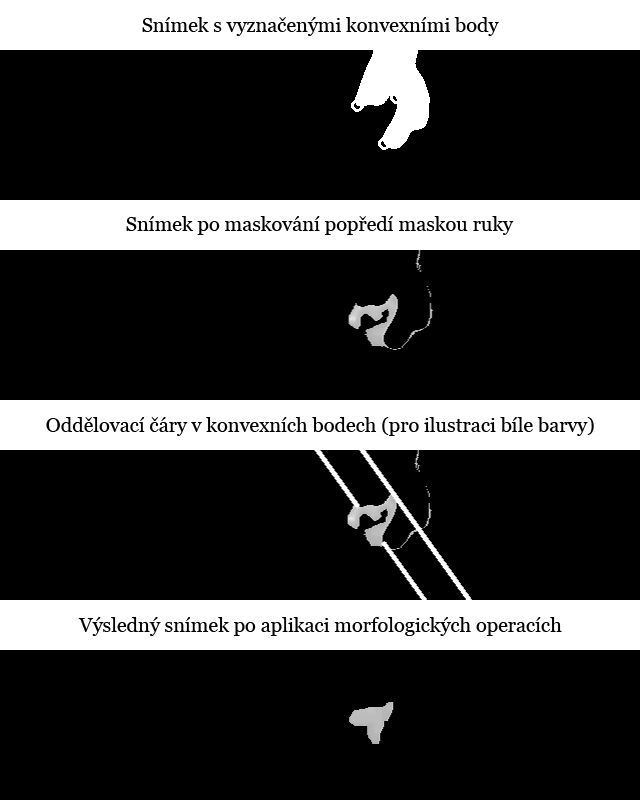
\includegraphics[width=0.8\textwidth]{images/camera_2_mog_goods_processing.png}
  \caption{Proces zpracování snímku zboží}
  \label{fig:camera_2_mog_goods_processing}
\end{figure} 

Na oddělené fragmenty obrazu jsou dále v~několika krocích vhodně aplikovány morfologické operace a to eroze a poté dilatace. Tento snímek může být zbylé zboží nebo šum a jsou na něm vypočteny předem dané atributy pro klasifikaci. Algoritmus je taktéž popsán ve vývojovém diagramu \ref{fig:edge_detection_diagram}. 

\begin{figure}[h]
  \centering
  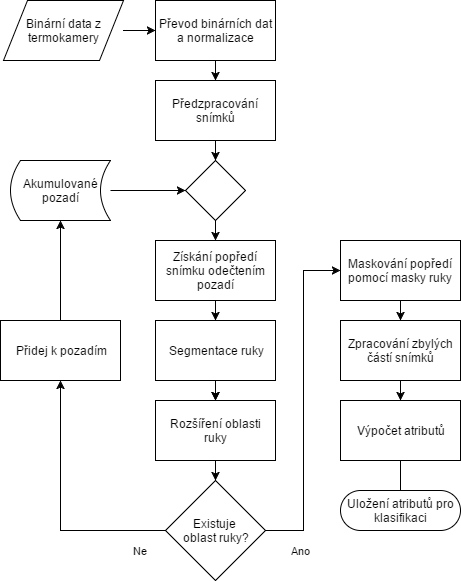
\includegraphics[width=0.8\textwidth]{images/mog_detection_diagram.png}
  \caption{Vývojový diagram algoritmu dynamického odečítání pozadí}
  \label{fig:mog_detection_diagram}
\end{figure} 

	\subsection{Úskalí řešení} \label{section:background_substract_problems}
    Největší nevýhodou tohoto řešení je, že je silně závislé na uloženém pozadí v~paměti. V~případě, že proběhne NUC kalibrace a do paměti se nestačí načíst dostatečný počet snímků nového pozadí, proběhne operace odečtení pozadí chybně. V~tomto případě jsou pak vypočteny nesmyslné hodnoty atributů, protože se jako zboží  tváří skoro celá oblast snímku. Pro ilustraci je tento případ zobrazen v~obrázku \ref{fig:camera_2_apply_mog_after_nuc}.
    
    Dalším problémem je, stejně jako v~algoritmu \ref{section:edge_detection_solution}, rychlý pohyb ruky při kterém se projevuje pohybová neostrost, která rozšiřuje pomyslnou oblast zboží.
    
    \begin{figure}[h]
      \centering
      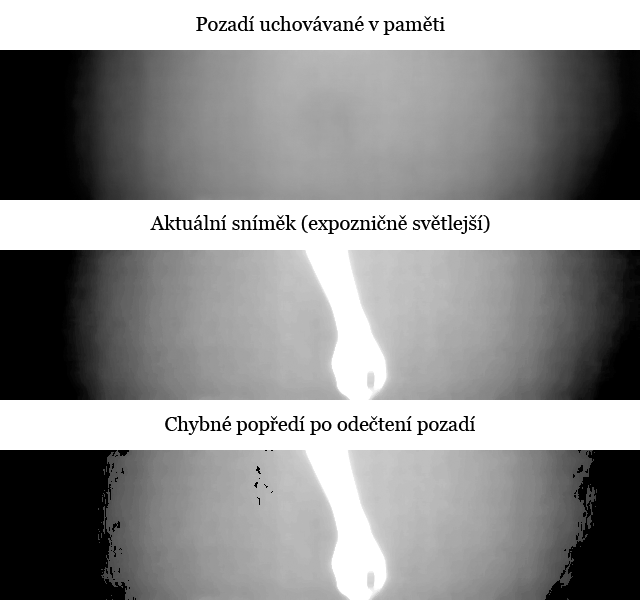
\includegraphics[width=0.8\textwidth]{images/camera_2_apply_mog_after_nuc.png}
      \caption{Chybně získané popředí kvůli změně expozice aktuálního snímku}
      \label{fig:camera_2_apply_mog_after_nuc}
	\end{figure} 

	\subsection{Vyhodnocení}
    Toto řešení bylo vybráno jako finální a jeho vyhodnocení je možné detailněji nalézt v~následující kapitole \ref{chapter:choosen_solution}.
    
\clearpage

\section{Řešení s~kombinací RGB obrazu}\label{section:combining_rgb_and_thermal}
U~všech řešení pouze s~termokamerou je největším problémem rozlišit pozadí (podlahu) od zboží kvůli velmi podobným teplotám a záři, která vzniká kolem ruky. V~případě, že by bylo možné striktně oddělit pozadí od popředí (ruka se zbožím), celý problém by se značně zjednodušil, protože segmentovat zboží od ruky lze díky rozdílným teplotám velmi snadno. 

V~tomto ohledu by bylo lepší využít klasickou kameru s~viditelným spektrem pro získání masky popředí. Tuto masku pak aplikovat na termovizní snímek a následně na něm segmentovat ruku a detekovat zboží. Tento snímek pak ještě vhodně zpracovat a vypočítat na něm atributy ke klasifikaci.

Pro otestování tohoto řešení byla využita externí RGB webkamera a ukázalo se, že toto řešení přináší dva velmi podstatné problémy.

    \subsection{Synchronizace kamer}
    Prvním problémem je sladění snímků z~různých kamer. Kamery spolu nejsou nijak propojeny a tak procesorové hodiny tikají na každé kameře jinak. Pořizované snímky v~čase jsou rozdílné a je možné nalézt snímky, které při pohybu ruky neodpovídají žádným snímkům z~druhé kamery. Jednoduše řečeno, kamery nemají synchronizované snímání a tak je u~každé kamery snímek vyhotoven v~jiný čas. Navíc u~toho u~termokamery vstupuje kalibrace NUC, při které kamera žádné snímky nepřenáší a občas se objevují i chyby přenosu, kdy požadovaný snímek nemusí být vůbec obdržen. 

    Snímky nelze přesně synchronizovat již po přijmutí z~kamer, protože by tímto způsobem vznikalo mnohem více chyb a výsledný algoritmus by byl méně přesný než v~případě jedné kamery.

    Synchronizaci snímků je možné řešit pouze hardwarově. Některé průmyslové kamery bývají vybaveny konektory, které slouží právě k~synchronizaci více kamer. Je možné propojit několik kamer, kdy synchronizace snímání probíhá vůči jedné vybrané kameře (master, slave režim). Synchronizaci je možné konfigurovat pomocí protokolu GenICam. Termokamera dostupná v~práci má k~dispozici synchronizační konektor, ale nebyla k~dispozici druhá kamera, která by s~ní byla kompatibilní.

	\subsection{Perspektiva snímků}
    Druhým problémem je rozdílná perspektiva snímků. Různé kamery nikdy nebudou mít stejnou optickou soustavu. Tento fakt je způsoben různými optickým vadami objektivů a často se objektivy liší i v~ohniskové vzdálenosti. Tyto skutečnosti pak ovlivňují výsledné zarovnání snímků. Na obrázku \ref{fig:webcam_sample} lze nejdříve vidět rozměrově neupravený snímek z~webkamery, který je následně oříznutý na oblast termokamery \ref{fig:visible_cropped_to_thermal}. V~posledním obrázku \ref{fig:visible_thermal_combined} jsou oba snímky prolnuty a lze snadno pozorovat, že i přes stejnou scénu na sebe snímky, právě díky rozdílné perspektivě, nelze přesně zarovnat.

    \begin{figure}[h]
      \centering
      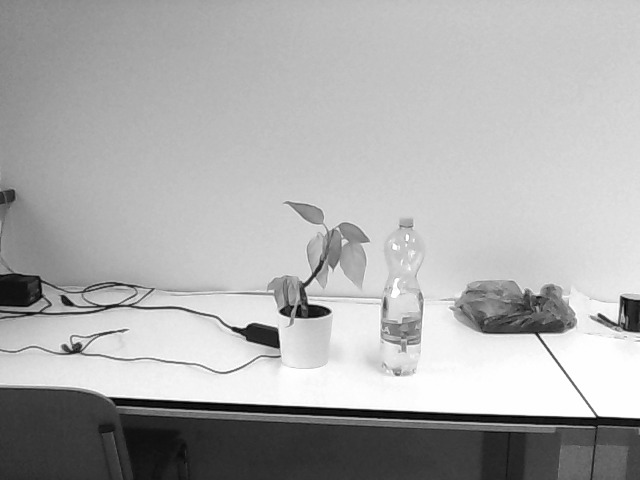
\includegraphics[width=0.6\textwidth]{images/webcam_sample.png}
      \caption{Ukázkový snímek snímaného obrazového pole webkamery}
      \label{fig:webcam_sample}
    \end{figure} 

    \begin{figure}[h]
      \centering
      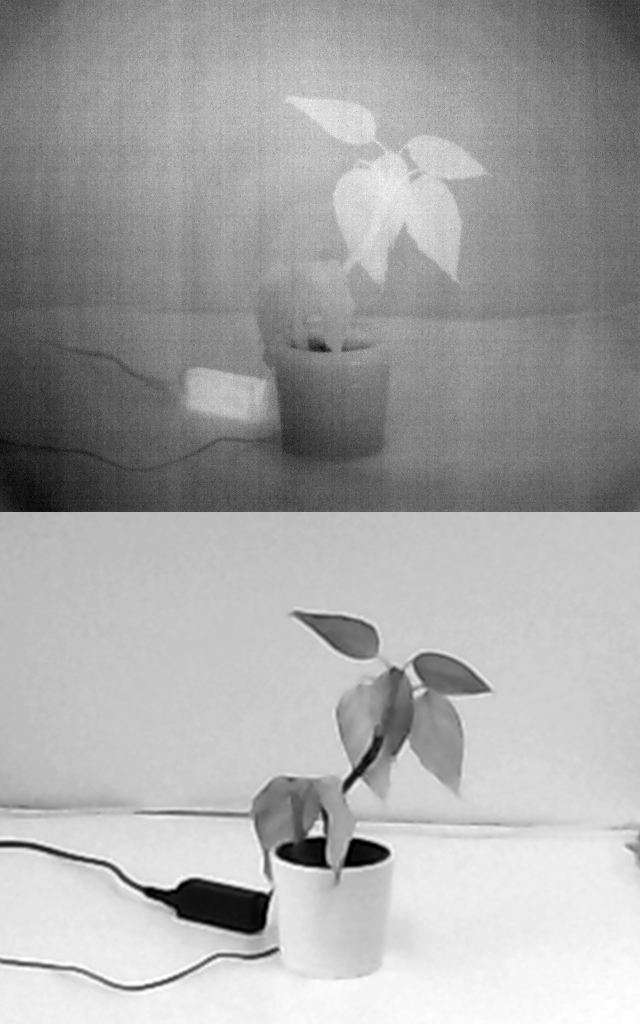
\includegraphics[width=0.6\textwidth]{images/visible_cropped_to_thermal.png}
      \caption{Snímek z~webkamery oříznutý k~obrazovému poli termokamery}
      \label{fig:visible_cropped_to_thermal}
    \end{figure} 

    \begin{figure}[h]
      \centering
      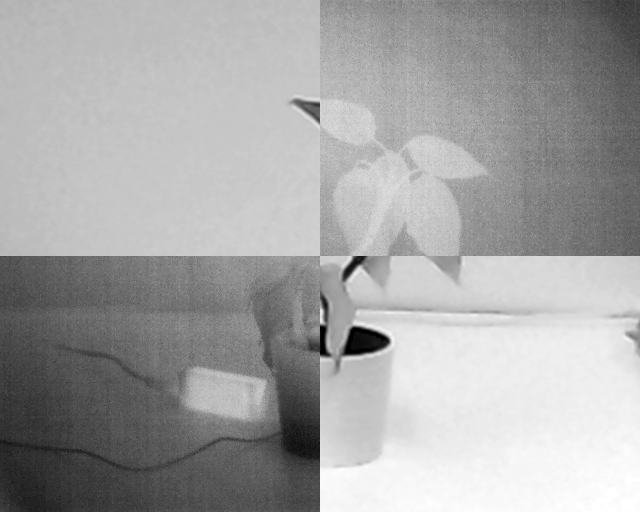
\includegraphics[width=0.9\textwidth]{images/visible_thermal_combined.png}
      \caption{Ručně sloučené snímky z~webkamery a termokamery}
      \label{fig:visible_thermal_combined}
    \end{figure} 

    Řešením je nalezení transformační matice homografie pro mapování obrazu webkamery na plochu obrazu termokamery. V~problému detekce zboží v~ruce to znamená hledání několika transformačních matic, protože perspektiva se mění v~závislosti na vzdálenosti snímaného objektu a ruka na snímku se může objevit v~několika rovinách. Čím více je nalezeno transformačních matic pro různé vzdálenosti, tím jsou výsledky mapování přesnější. V~knihovně OpenCV je hledání transformační matice homografie již implementováno metodou findHomography z~balíku calib3d.

	\subsection{Shrnutí}
    Toto řešení nakonec nebylo implementováno hlavně kvůli problémům se synchronizací kamer, které v~rámci práce nebylo možné vyřešit. Pro případné navázaní na tuto práci je alespoň uveden vývojový  diagram \ref{fig:visible_thermal_detection_diagram} algoritmu.

    \begin{figure}[h]
      \centering
      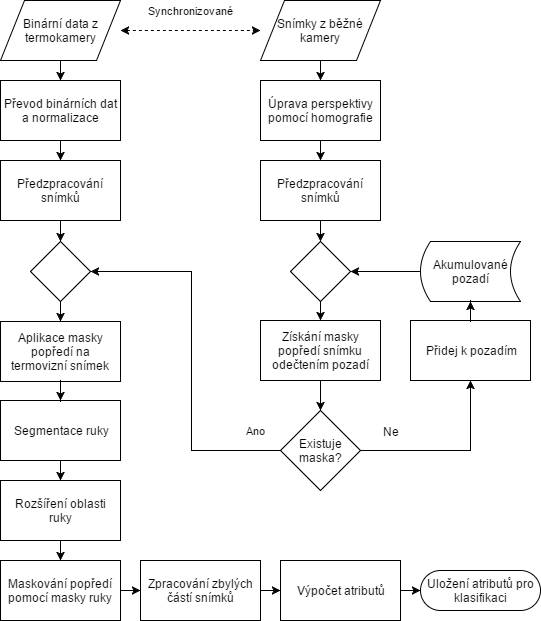
\includegraphics[width=0.9\textwidth]{images/visible_thermal_detection_diagram.png}
      \caption{Vývojový diagram algoritmu využívající kombinace běžného a termografického snímku}
      \label{fig:visible_thermal_detection_diagram}
    \end{figure} 


    



